\documentclass[10pt]{beamer}

\usepackage{siunitx}
\usepackage[normalem]{ulem}
\usepackage{multirow,bigdelim}
\usepackage{empheq}
\newcommand*{\UTALATEXPATH}{latex/}
      \usepackage{\UTALATEXPATH atlasmisc}
      \usepackage{\UTALATEXPATH atlasmath}
      \usepackage{\UTALATEXPATH atlasparticle}
      \usepackage{\UTALATEXPATH atlasphysics}
      \usepackage{\UTALATEXPATH atlasprocess}
      \usepackage{\UTALATEXPATH atlasbsm}
      \usepackage{\UTALATEXPATH atlasheavyion}
      \usepackage{\UTALATEXPATH graphicx} % to insert PostScript figures
\usepackage[many]{tcolorbox}
\definecolor{babyblue}{rgb}{0.54,0.81,0.94}
\definecolor{kugray5}{RGB}{224,224,224}
\definecolor{light-gray}{gray}{0.75}


\tcbset{colframe=white,colback=white,nobeforeafter}
\tcbset{highlight math style={enhanced,
  colframe=red!60!black,colback=yellow!50!white,arc=4pt,boxrule=1pt,
  }}

\newtcbox{\mybox}[1][]{nobeforeafter,math upper,tcbox raise base,
  enhanced,frame hidden,boxrule=0pt,interior style={top color=green!10!white,
  bottom color=green!10!white,middle color=green!50!yellow},
  fuzzy halo=1pt with green,drop large lifted shadow,#1}

\usetheme[progressbar=frametitle]{metropolis}

\usepackage{booktabs}
\usepackage[scale=2]{ccicons}
\usepackage{outlines}
\usepackage{multicol}
\usepackage{pgfplots}
\usepgfplotslibrary{dateplot}
\usepackage{hyperref}
\usepackage{psfrag}

\usepackage{xspace}

%%%%%%%%%%%%%%%%%%%%%%%%%%%%%%%%%%%%%%%%%%%%%%%%%%%%%%%%%%%%%%%%%%
% Some new commands
%%%%%%%%%%%%%%%%%%%%%%%%%%%%%%%%%%%%%%%%%%%%%%%%%%%%%%%%%%%%%%%%%%

\newcommand\Fontvi{\fontsize{9}{9}\selectfont}
\newcommand{\rectangle}[2]{{% #1 = width, #2 = height
  \fboxsep=-\fboxrule\sbox0{}\wd0=#1\ht0=#2\relax\fbox{\box0}}}

\newcommand{\reftemp}[1]{#1}

\def\checkmark{\tikz\fill[scale=0.3](0,.35) -- (.25,0) -- (1,.7) -- (.25,.15) -- cycle;} 
\newcommand{\themename}{\textbf{\textsc{metropolis}}\xspace}
\newcommand*{\yyWW}{\ensuremath{\gamma\gamma \to W^+W^-}}
\newcommand*{\yyll}{\ensuremath{\gamma\gamma \to \ell^+\ell^-}}
\newcommand*{\yymumu}{\ensuremath{\gamma\gamma \to \mu^+\mu^-}}
\newcommand*{\yyee}{\ensuremath{\gamma\gamma \to e^+e^-}}
\newcommand*{\yytautau}{\ensuremath{\gamma\gamma \to \tau^+\tau^-}}
\newcommand*{\gamgamWWll}{\ensuremath{\gamma\gamma \to W^+W^- \to \ell^{+} \nu \ell'^{-} \bar{\nu}}}
\newcommand*{\ggHWWll}{\ensuremath{gg\ra H \ra W^+W^- \ra \ell^{+} \nu \ell'^{-} \bar{\nu}}}
\newcommand*{\HWWll}{\ensuremath{gg\ra H \ra W^+W^- \ra \ell^{+} \nu \ell'^{-} \bar{\nu}}}
\newcommand*{\DrellYantomumu}{\ensuremath{Z/\gamma^* \to \mu^+\mu^-}}
\newcommand*{\DrellYantotautau}{\ensuremath{Z/\gamma^* \to \tau^+\tau^-}}
\newcommand*{\ggww}{\textsc{gg2ww}\xspace}
\newcommand*{\tauvis}{\ensuremath{\tau_{\text{had-vis}}}}
\newcommand*{\cHtaunu}{\ensuremath{H^+ \to \tau^+\nu}}
\newcommand*{\Wjets}{\ensuremath{W+\text{jets}}}
\newcommand*{\Zjets}{\ensuremath{Z+\text{jets}}}
\newcommand*{\FF}{\ensuremath{\text{FF}}}
\newcommand*{\WW}{\ensuremath{W^+W^-}} %%
\newcommand*{\mmumu}{\ensuremath{m_{\mu\mu}}}

\newcommand*{\PowhegPythiaEight}{\textsc{Powheg+Pythia8}\xspace}
\newcommand*{\AlpgenPythiaSix}{\textsc{Alpgen+Pythia6}\xspace}
\newcommand*{\AlpgenHerwig}{\textsc{Alpgen+Herwig}\xspace}
\newcommand*{\PYTHIAsix}{\textsc{Pythia6}\xspace}

\newcommand*{\pTll}{\ensuremath{p_{\textrm{T}}^{\ell\ell}}}
\newcommand*{\pTemu}{\ensuremath{p_{\textrm{T}}^{e\mu}}}
\newcommand*{\pTmumu}{\ensuremath{p_{\textrm{T}}^{\mu\mu}}}
\newcommand*{\mll}{\ensuremath{m_{\ell\ell}}}
\newcommand*{\memu}{\ensuremath{m_{e\mu}}}
%\newcommand*{\mT}{\ensuremath{m_{\textrm{T}}}}
\newcommand*{\dFll}{\ensuremath{\Delta\phi_{\ell\ell}}}
\newcommand*{\dFem}{\ensuremath{\Delta\phi_{e\mu}}}
\newcommand*{\Ztau}{\ensuremath{Z\to\tau\tau}}
\newcommand*{\DZ}{\ensuremath{\Delta z_0^{\mathrm{iso}}}}
\newcommand*{\fEL}{\ensuremath{f_{\mathrm{EL}}}}
\newcommand*{\fgam}{\ensuremath{f_{\gamma}}}
%\newcommand*{\fP}{\ensuremath{f^{\mathrm{P}}}}
%\newcommand*{\fAP}{\ensuremath{f^{\mathrm{AP}}}}
%\newcommand*{\fAH}{\ensuremath{f^{\mathrm{AH}}}}
%\newcommand*{\LambdaCutoff}{\ensuremath{\Lambda_{\textrm{cutoff}}}}
%\newcommand*{\BR}{\textrm{BR}}

\setbeamercolor{alerted text}{fg=blue,bg=white}
\setbeamercolor{background canvas}{bg=white}

\title{Search for exclusive and charged Higgs bosons}
\subtitle{with ATLAS at the LHC}
\date{\today}
\author{Last Feremenga, {\footnotesize Supervised by: Jaehoon Yu}\\ Ph.D Thesis Defense}
\institute{University of Texas at Arlington}
\titlegraphic{
\includegraphics[height=1.5cm]{figures/UTA_A-logo_Sml_2c-pms.eps}\hfill\includegraphics[height=1.5cm]{figures/AT_atlaslogo_2015.eps}\hfill\includegraphics[height=1.5cm]{figures/AT_cernlogo.eps}}

\begin{document}

\maketitle

\begin{frame}{Table of contents}
  \setbeamertemplate{section in toc}[sections numbered]
  \tableofcontents[hideallsubsections]
\end{frame}

\section{Introduction}

\begin{frame}{The Standard Model (SM)}
\centering
 {\color{blue}\large SM summarizes current understanding of matter and forces} 
\begin{figure}
\centering
\includegraphics[width=0.7\linewidth]{figures/sm.png}
\end{figure}
Also successful in making predictions
\end{frame}


\begin{frame}{SM -- experiments}
\centering
{\color{blue}\large Tested through scattering experiments -- e.g proton scattering} 
\vspace*{-0.5\baselineskip}
\begin{outline}
\1 Protons made up of quarks and gluons (partons) 
	\2 Proton collision $\rightarrow$ parton collision
\1 Primary parton hard scatter expected to produce interesting physics
	\2 Proton remnant activity referred to as  {\color{purple} underlying events (UE)} 
\end{outline}
\begin{figure}
\includegraphics[width=0.8\linewidth]{figures/collision.pdf}
\end{figure}
\begin{outline}
\1 \uline{Bunches} of protons collided to maximize probability of collision 
\1 Multiple proton collisions per bunch 
	\2 One primary and multiple {\color{purple} pile-up} collisions
\end{outline}
\end{frame}

\begin{frame}{SM Higgs boson -- discovery and future prospects}
Higgs boson discovered in 2012 -- updated $\mH=125.09\pm0.24$~\GeV
\vspace*{-0.5\baselineskip}
\begin{figure}
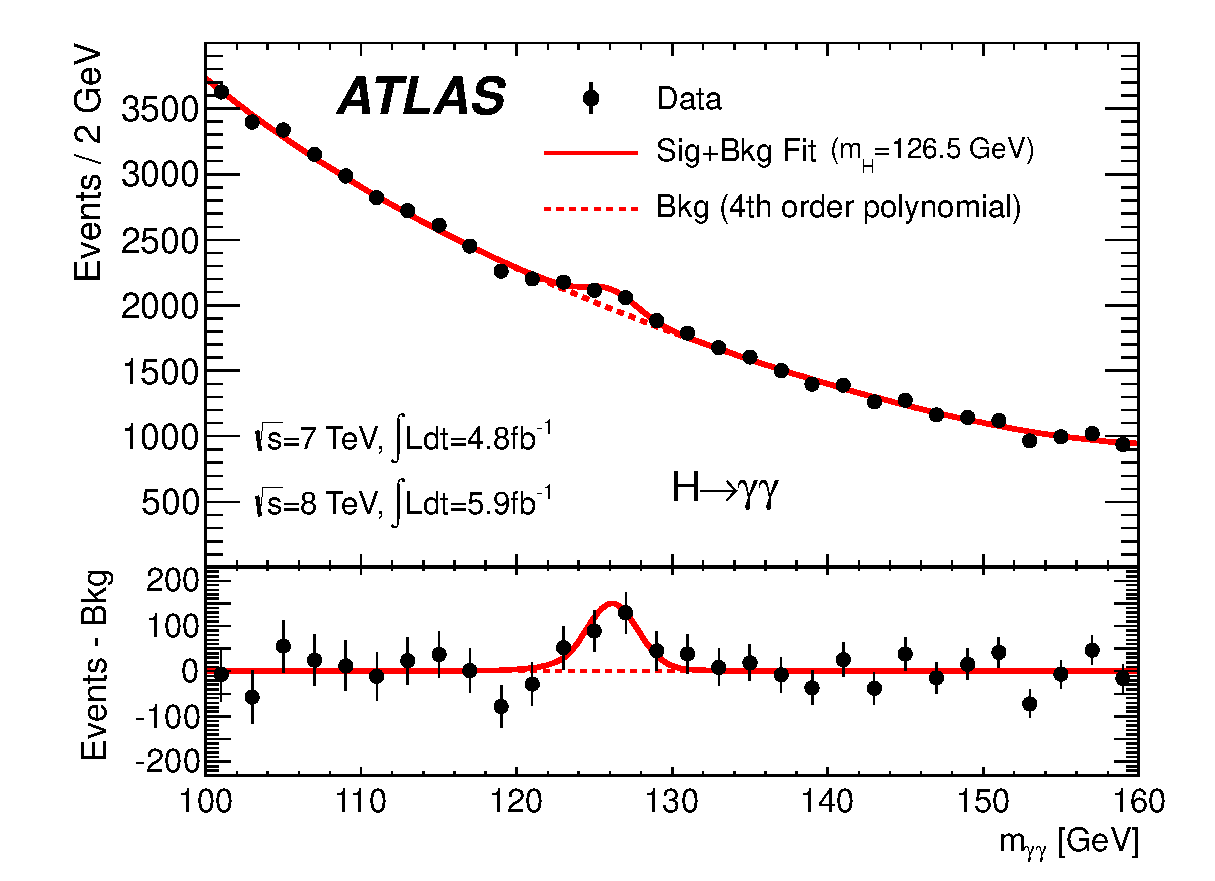
\includegraphics[width=0.7\linewidth]{figures/figaux_004a.eps}
\end{figure}
\vspace*{-1.2\baselineskip}
Efforts towards precision studies on its properties:
\vspace*{-0.5\baselineskip}
\begin{outline}
\1 Coupling constants, quantum numbers, invisible decays
\end{outline}
{\color{blue}\large Analysis channels with minimal backgrounds necessary}
\end{frame}

\begin{frame}{Exclusive Production -- Candidate for precision studies}
\centering
{\large\color{blue} Exclusive processes have very little background contamination}
\vspace*{-0.5\baselineskip}
\begin{figure}
\centering
\includegraphics[width=0.6\linewidth]{figures/diffraction.pdf}
\end{figure}
\vspace*{-0.5\baselineskip}
\begin{outline}
\1 Scattering protons effectively do not exchange quantum numbers
\1 Only share momentum during collision
	\2 Shared momentum could create the SM Higgs boson
\1 No underlying event $\rightarrow$ cleanliness 
\end{outline}
%a.k.a {\bf exclusive} because Higgs boson is produced with nothing else 

\centering
{\bf\large \color{blue} Thesis Project I}\\
\tcbox[colback=white,colframe=blue,nobeforeafter,tcbox raise base,top=0pt,left=0pt,right=0pt,bottom=0pt]{
{\large Search for evidence of exclusive Higgs boson}
}

\end{frame}

\begin{frame}{Shortfalls of the SM}
\begin{quote}
``Failure is not fatal, but failure to change might be." \par\raggedleft -- \textup{John Wooden}
\end{quote}
\begin{outline}
\1 Absence of gravity 
\1 Massless neutrinos
\1 Dark matter candidates
\1 CP violation in cosmology
\1 {\bf Hierarchy problem -- large differences in coupling constants at low energy scales} 
\end{outline}
\begin{columns}
	\begin{column}{0.5\linewidth}
{\color{blue} Hierarchy problem could be addressed by SUperSYmmetric (SUSY) theories}
	\end{column}
	\begin{column}{0.5\linewidth}
\includegraphics[width=\linewidth]{figures/susyparticles.jpg}
	\end{column}
\end{columns}
\end{frame}

\begin{frame}{Minimal Supersymmetric extension to Standard Model (MSSM)}
Higgs sector now comprises 5 Higgs bosons:
\begin{outline}
\1 light Higgs, \hzero -- scalar
	\2 if \hzero is taken as the SM Higgs, MSSM is known as {\bf hMSSM}
\1 heavy Higgs, \Hzero -- scalar
\1 neutral Higgs, \Azero -- pseudo-scalar, CP-odd
\1 {\bf charged Higgs}, \Hpm -- scalar 
\end{outline}
\noindent\makebox[\linewidth]{\rule{\paperwidth}{0.4pt}}
Built on two Higgs doublet fields, rather than one Higgs field 
%The Two-Higgs-Doublet Model (2HDM), built on two Higgs doublet fields, corresponds to hMSSM
\begin{outline}
\1 Entire parameter space of Higgs sector can be parametrized by:
		\2 $\tan\beta$ -- ratio of vacuum expectation 
values of the two Higgs doublets
		\2 $\mcH$ -- mass of \Hpm
\end{outline}

\centering
{\bf \color{blue}\large Thesis Project II}\\
\tcbox[colback=white,colframe=blue,nobeforeafter,tcbox raise base,top=0pt,left=0pt,right=0pt,bottom=0pt]{
{\large Search for evidence of charged Higgs boson}
}
\end{frame}

\section{The Experiment}

\begin{frame}{The Large Hadron Collider (LHC)}
\centering
 27 km-long accelerator colliding bunches of protons
\includegraphics[width=\linewidth]{figures/lhc-sim.jpg}
\vspace*{-1.5\baselineskip}
\begin{table}[!h]
\centering
  \resizebox{\textwidth}{!}{
   \begin{tabular}{|l|ccc|}
\hline
 Parameter           								& Run I Value    & Run II Value & Design Value \\
\hline\hline
Beam Energy [\TeV]   								&          4     &  	6.5       &    7         \\
Bunch spacing [\SI{}{\nano\second}] & 				50 		 & 		25 				& 	25 				 \\
Protons per bunch										&\num{1.7e11}    & \num{1.18e11}& \num{1.15e11}\\
Average pile-up       							&  20.7            &  22.9          & 20    \\ 
\hline
   \end{tabular}
}
\label{tab:lhcParas}
\end{table}
Has had 2 long runs : Run I (2011$\to$2012) and Run II (2015$\to$2016)
\end{frame}


\begin{frame}{The LHC -- Deliverables}
\centering
{\large\color{blue} Goal is to optimally produce rare processes} 
\begin{outline}
\1 Performance quantified by {\color{blue} instantaneous luminosity},
\end{outline}
\vspace*{-0.8\baselineskip}

\begin{empheq}[box=\mybox]{align}
\nonumber L = N_{process}/\sigma_{process}
\end{empheq}

\begin{columns}
	\begin{column}{0.5\linewidth}
   \includegraphics[width=\textwidth]{figures/peakLumiByFill2012.png}
	\end{column}
	\begin{column}{0.5\linewidth}
   \includegraphics[width=\textwidth]{figures/peakLumiByFill.png}
	\end{column}
\end{columns}

\begin{outline} 
\1 {\color{blue} Integrated luminosity} $\mathcal{L} = \int_0^{T} L dt$ over time $T$ quoted to correspond data collected 
\end{outline} 

\end{frame}

\begin{frame}{A Toroidal LHC ApparatuS (ATLAS)}
\centering
{\large\color{blue} Large all-purpose detector built around LHC collision point}
\begin{figure}
\centering
   \includegraphics[width=0.9\textwidth]{figures/figures_AtlasDetectorLabelled.png}
\end{figure}
\vspace*{-\baselineskip}
\begin{outline}
\1 Precision charged particle tracking
\1 Momentum and energy reconstruction
\end{outline}
\end{frame}

\begin{frame}{ATLAS -- particle detection}
\begin{figure}
\centering
   \includegraphics[width=0.9\textwidth]{figures/CL_fig1.jpg}
\end{figure}
\end{frame}

\begin{frame}{ATLAS -- coordinate system}
\centering
Cylindrical coordinate system
\begin{figure}
	\centering
   \includegraphics[width=0.9\textwidth]{figures/Figures_T_Coordinate.png}
	\label{fig:coord}
\end{figure}
\begin{outline}
\1 Transverse plane  $\longrightarrow$ ($r,\phi$) 
\1 Longitudinal plane $\longrightarrow$ pseudo-rapidity $\eta=-\ln\tan(\theta/2)$
\1 Metric $\longrightarrow$ angular distance $\Delta R = \sqrt{(\Delta\eta)^2 + (\Delta\phi)^2}$
\end{outline}
\end{frame}

\begin{frame}{ATLAS -- trigger system}
Not all data can be collected and saved to disk; available space has limits
\begin{figure}
	\centering
   \includegraphics[width=0.9\textwidth]{figures/trigger.png}
\end{figure}
\begin{outline}
\1 Bunch crossing rate reduced from {\bf $\sim$ 40~MHz} to about {\bf $\sim$ 200~Hz}
\1 L2 and Event Filter combined into Higher Level Trigger (HLT) in Run II 
\end{outline}
\end{frame}

\section{Search for exclusive Higgs boson}

\begin{frame}{Production}
\centering
{\large\color{blue} Protons remain intact after collision }\\
%
%\begin{equation*}
%\sigma_{pp(gg)\ra ppH} \propto \hat{\sigma}(gg\ra H)\left ( \int \frac{dQ^2_t}{Q^4_t}f_g(x_1, x_1^{'},Q^2_t)f_g(x_2, x_2^{'},Q^2_t)\right )^2 
%\end{equation*}
%
%\begin{columns}
%	\begin{column}{0.5\linewidth}
%\begin{outline}
%\1 Underlying process is the standard gluon fusion
%\1 Extra gluon exchanged maintains color in original protons
%\end{outline}
%	\end{column}
%	\begin{column}{0.5\linewidth}
\begin{figure}
\centering
\includegraphics[width=0.8\linewidth]{figures/exclH.pdf}
\end{figure}
%	\end{column}
%\end{columns}
\begin{outline}
\1 Higgs dominantly produced through standard gluon fusion
\1 Extra gluon exchanged maintains color in original protons
\1 Predicted 3 fb total production cross section at 8~\TeV\ LHC
%	\2{\bf Project} : Put this and other hypotheses to test using Run I ATLAS data
\end{outline}
\end{frame}

\begin{frame}{Decay channels}
\begin{columns}
	\begin{column}{0.5\linewidth}
\begin{outline}
\1 Largest branching ratios:
	\2 $H\to b\bbar$
	\2 $H\to\WW$ 
\1 Too much QCD multi-jets bkg. in $b\bbar$
	\2 Multi-jets too complex to model correctly
\1 \WW\ is the optimal choice 
\1 \Wpm\ decay to leptons of different flavor, and charge
\end{outline}
	\end{column}
	\begin{column}{0.5\linewidth}
\begin{figure}
\centering
   \includegraphics[width=\textwidth]{figures/Higgs_BR_LM.eps}
\end{figure}
	\end{column}
\end{columns}
\centering
{\color{blue}\large Complete decay channel : \HWWll} 
\end{frame}

\begin{frame}{Major background processes}
\centering 
{\large\color{blue} Backgrounds separated into inclusive and exclusive}

\vspace*{\baselineskip}

\begin{tcolorbox}[title=Inclusive Backgrounds, width=\linewidth, colback=white,colframe=cyan,nobeforeafter,tcbox raise base,top=0pt,left=0pt,right=0pt,bottom=0pt]
\begin{outline}
	\1 {\bf Inc. $\boldsymbol{WW}$}: Non-diffractive direct production of \WW
	\1 {\bf Top}: \ttbar\ and single top
	\1 {\bf VV}: Non-diffractive direct production of $WZ,ZZ,W\gamma, Z\gamma$ 
	\1 {\bf V+jets}: Non-diffractive direct production of $W/Z$+jets
\end{outline}
\end{tcolorbox}
\vspace*{\baselineskip}
\begin{tcolorbox}[title=Exclusive Backgrounds, width=\linewidth, colback=white,colframe=red!50!white,nobeforeafter,tcbox raise base,top=0pt,left=0pt,right=0pt,bottom=0pt]
\begin{outline}
	\1 {\bf Excl. $\boldsymbol{WW}$}: Exclusive production of \WW
	 \2 E.g \yyWW
	\1 {\bf Excl. $\boldsymbol{ll}$}: Exclusive and direct production of $ll$
	 \2 E.g \yyll  
\end{outline}
\end{tcolorbox}
\end{frame}

\begin{frame}{Major exclusive backgrounds}
\centering
{\color{blue}\large Exclusive backgrounds come in many forms!}
\vspace*{\baselineskip}
\begin{columns}
	\begin{column}{0.33\linewidth}
	\centering
	Elastic
   \includegraphics[width=\textwidth]{figures/exclWW.pdf}
	\end{column}
	\begin{column}{0.33\linewidth}
\centering
Single Dissociative (SD)
   \includegraphics[width=\textwidth]{figures/exclWWsd.pdf}
	\end{column}
	\begin{column}{0.33\linewidth}
\centering
Double Dissociative (DD)
   \includegraphics[width=\textwidth]{figures/exclWWdd.pdf}
	\end{column}
\end{columns}
\begin{outline}
\1 In all cases, proton remnants outside detector fiducial space 
\1 Excl. $ll$ production identical to excl. $WW$ 
\1 SD and DD difficult to model with MC
	\2 Estimated with data-driven methods
\end{outline}
\end{frame}

\begin{frame}{Event Selection [Signal region (SR) definition]}
\centering
{\color{blue}\large $gg\to[H]\to[\Wplus][\Wminus]\to[l][l][\met]$}

\vspace*{\baselineskip}

\begin{columns}
	\begin{column}{0.5\linewidth}
\begin{outline}
\1 Lower bound on lepton \pt\ suppresses QCD and \Wjets 
\1 Lower bound on \memu\ suppresses QCD and Drell-Yan 
\1 Upper bound on \memu\ exploits Higgs spin-0
	\2 Same as \dFem
\1 $\pTemu$, suppresses QCD multijets, $V$+jets and 
\end{outline}
	\end{column}
	\begin{column}{0.5\linewidth}
\begin{tcolorbox}[title=Signal Selection, width=\linewidth, colback=white,colframe=red!50!white,nobeforeafter,tcbox raise base,top=0pt,left=0pt,right=0pt,bottom=0pt]
\begin{enumerate}
\item Oppositely charged $e\mu$   
\item   $\pT^{\ell 1} > 25$, $\pT^{\ell 2} > 15\GeV$ 
\item  $10< \memu <55\GeV$    
\item $\pTemu > 30\GeV$
\item $\dFem < 1.8$       
\item $\mT <140$~\GeV       
\item Exclusivity selection, \DZ
\end{enumerate}
\end{tcolorbox}
	\end{column}
\end{columns}
%\vspace*{\baselineskip}
%\begin{outline}
%\1 {\bf pre-selection}: Selections 1$\to$4 without $\memu<55\GeV$
%\end{outline}
\end{frame}

\begin{frame}{Exclusivity Selection, \DZ}
\centering
{\large\color{blue} Exploit large gaps btwn protons and dilepton system}\\
{\large\color{red} Expect no tracks in the large gaps}
\begin{columns}
	\begin{column}{0.5\linewidth}
   \includegraphics[width=\textwidth]{figures/cartoon.eps}
	\end{column}
	\begin{column}{0.5\linewidth}
 \includegraphics[width=\linewidth]{figures/muFit.eps} 
	\end{column}
\end{columns}
\begin{outline}
\1 For inclusive processes, expect extra tracks 
	\2 Extra tracks from underlying event 
\1 Optimal $\DZ=1$ mm,  $\epsilon = 58\pm 6\%$, rejection $=\mathcal{O}(10^3)$
\end{outline}
\end{frame}

\begin{frame}{\DZ, validation}
\centering
{\large\color{blue} MC known to overestimate elastic $\gamma\gamma\to X$ (\href{http://arxiv.org/abs/1410.2983}{arxiv 1410.2983})}
\begin{outline}
\1 {\bf Strategy} : Derive scale factor \fEL\ from \yymumu\ data 
	\2 \fEL\ is ratio of observed elastic \yymumu\ to MC prediction 
\end{outline}
\begin{columns}
	\begin{column}{0.45\linewidth}
\begin{tcolorbox}[title=\yymumu\ Selection, width=\linewidth, colback=white,colframe=red!50!white,nobeforeafter,tcbox raise base,top=0pt,left=0pt,right=0pt,bottom=0pt]
\begin{enumerate}
\item 2 $\mu$ with $\pT^{\mu} > 20\GeV$
\item $45 < \mmumu < 75\GeV$ or $\mmumu>105\GeV$ 
\item $\pTmumu< 3$ GeV and $\DZ = 1.0$~mm 
\end{enumerate}
Drell-Yan only significant bkg
\end{tcolorbox}
\vspace*{-\baselineskip}
	\end{column}
	\begin{column}{0.55\linewidth}
\begin{figure}
\psfrag{variableX}{$1 - |\Delta\phi_{\mu\mu}|/\pi$}
\psfrag{Events / 0.001}{Events / 0.001}
 \includegraphics[width=\linewidth]{figures/dilepton_3shapes_Washington_filled.eps} 
\end{figure}
	\end{column}
\end{columns}
\begin{outline}
\1 Vary $\pTmumu$ and $\DZ$ to evaluate systematic uncertainties 
\end{outline}
\vspace*{-0.3\baselineskip}

\centering
\tcbox[colback=white,colframe=red!50!white,nobeforeafter,tcbox raise base,top=0pt,left=0pt,right=0pt,bottom=0pt]{
$\fEL = 0.76 \pm 0.04 (\textrm{stat.}) \pm 0.10 (\textrm{sys.})$
}\\
\vspace*{0.3\baselineskip}
\centering
Previous measurements cover between 0.73 and 0.75
\end{frame}

\begin{frame}{\DZ, Pileup robustness}
\centering
{\large\color{blue} Effect of pile-up on exclusivity selection must be quantified} 
\begin{outline}
\1 {\bf Strategy :} Evaluate $f=$ Data/(Elastic+SD+DD) in two data regions 
	\2 Nominal exclusivity vs. pile-up prone exclusivity
\end{outline}
\begin{columns}[T]
	\begin{column}{0.4\linewidth}
\begin{tcolorbox}[title={Nominal [$f=0.73$]}, width=\linewidth, colback=white,colframe=red!50!white,nobeforeafter,tcbox raise base,top=0pt,left=0pt,right=0pt,bottom=0pt]
Excl. $\mu\mu$ sel. except :
%\vspace*{-\baselineskip}
\begin{enumerate}
\item acoplanarity $<0.0015$ 
\item $\DZ = 1.0$~mm 
\end{enumerate}
\end{tcolorbox}
%\vspace*{1.5\baselineskip}
\begin{tcolorbox}[title={Pileup-prone [$f=0.70$]}, width=\linewidth, colback=white,colframe=cyan,nobeforeafter,tcbox raise base,top=0pt,left=0pt,right=0pt,bottom=0pt]
Similar to Nominal except :
\vspace*{-\baselineskip}
\begin{enumerate}
\item 1 extra track with $\DZ = 3.0$~mm
\end{enumerate}
\end{tcolorbox}
	\end{column}
	\begin{column}{0.6\linewidth}
 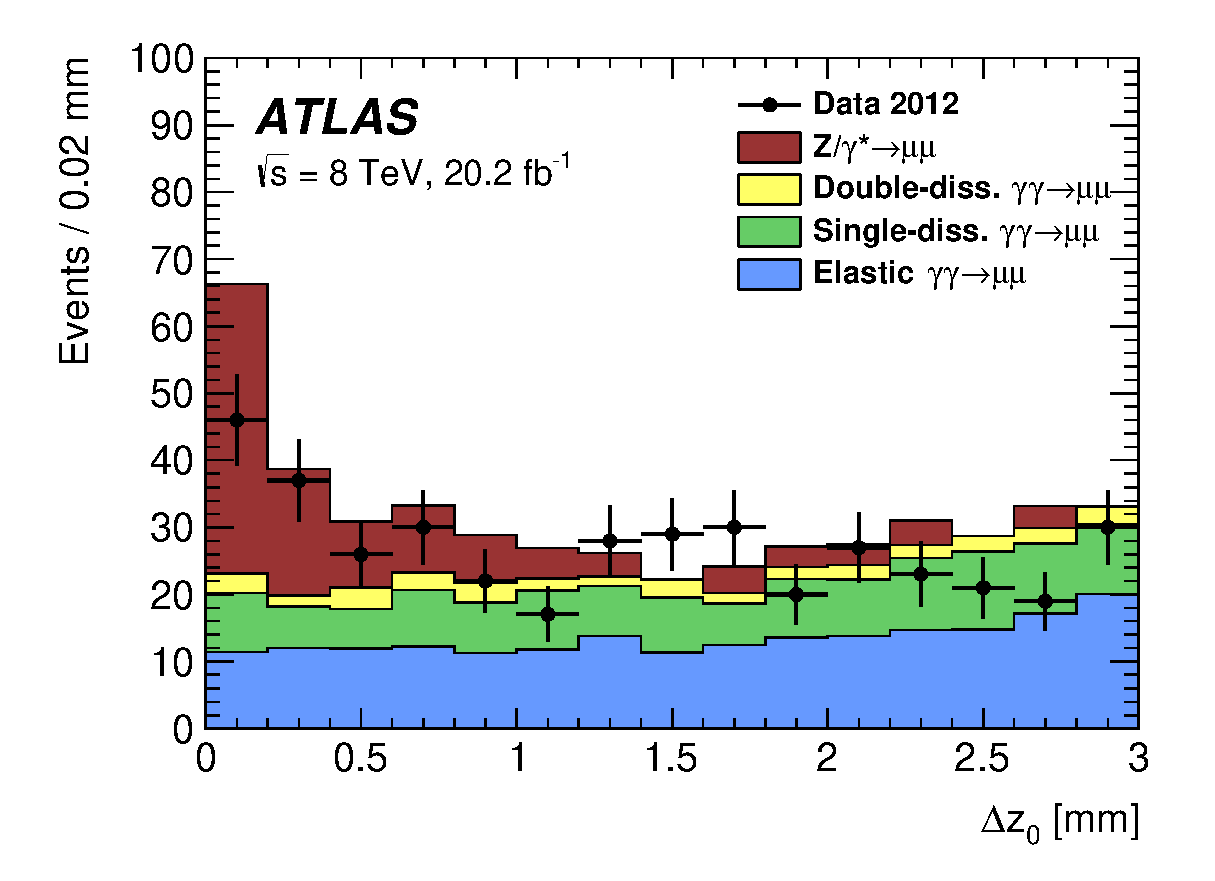
\includegraphics[width=\linewidth]{figures/dilepton_dzone6.eps} 
	\end{column}
\end{columns}
\begin{outline}
\1 2 scale factors compatible at 10\% $\Rightarrow$ syst. error due to pile-up is 10\%
\end{outline}
\end{frame}

\begin{frame}{Track Multiplicity in MC}
\centering
{\large\color{blue} Underlying event may not be modelled correctly in simulation} 
\begin{outline}
\1 {\bf Strategy : }  Extract scale factors ($\epsilon_{\textrm{Data}}/\epsilon_{\textrm{MC}}$) from Drell-Yan data 
\end{outline}
%\vspace*{-\baselineskip}
\begin{columns}
	\begin{column}{0.4\linewidth}
\begin{tcolorbox}[title=Selection, width=\linewidth, colback=white,colframe=red!50!white,nobeforeafter,tcbox raise base,top=0pt,left=0pt,right=0pt,bottom=0pt]
\yymumu\ \hyperlink{mumu}{selection} except :
\begin{enumerate}
\item $80 < m_{\mu\mu} < 100$~GeV 
\item No \pTmumu\ selection
\end{enumerate}
Exclusivity $\DZ = 1.0$~mm 
\end{tcolorbox}
	\end{column}
	\begin{column}{0.6\linewidth}
\begin{figure}
\psfrag{Events / 20 GeV}{Events / 20 GeV}
\psfrag{Data / MC}{Data / MC}
\psfrag{mass}{$m_{e\mu}$ [GeV]}
\includegraphics[width=\linewidth]{figures/zrejcal.eps}
\end{figure}
	\end{column}
\end{columns}

\begin{outline}
\1 Rejection more in $Z/\gamma\to\mu^+\mu^-$ data than MC
%\1 Scale factors are then validated in the region shown in the right hand plot, with $\memu<$ 90 GeV
\1 Systematics evaluated by varying MC generator across $\mmumu$ (20\%)
\end{outline}
\end{frame}


\begin{frame}{Estimation of SD and DD components}
\centering
{\large\color{blue} No simulation for SD and DD \yyWW}
%\vspace*{-\baselineskip}
\begin{columns}
	\begin{column}{0.5\linewidth}
\begin{outline}
\1 {\bf Strategy : }  Extract correction factor \fgam\ from excl. $\mu\mu$ data 
% \2 \yyWW\ estimate scaled by \fgam 
\end{outline}
\vspace*{-0.5\baselineskip}
%\begin{tcolorbox}[title=Selection, width=\linewidth, colback=white,colframe=cyan,nobeforeafter,tcbox raise base,top=0pt,left=0pt,right=0pt,bottom=0pt]
%\yymumu\ \hyperlink{mumu}{selection} except :
%\begin{enumerate}
%\item $m_{\mu\mu} > 160~\GeV$ 
%\item No \pTmumu\ selection
%\end{enumerate}
%Exclusivity $\DZ = 1.0$~mm 
%\end{tcolorbox}
%Corresponding \yyee\ selection also considered
\centering

\begin{empheq}[box=\mybox]{align}
\nonumber \fgam = \frac{\mathrm{N}_{\mathrm{Data}} 
              - \mathrm{N}^{\POWHEG}_{\mathrm{Background}}}{\mathrm{N}^{\HERWIGPP}_{\mathrm{Elastic}}}
            = 3.30
%            = 3.30 \pm 0.22 \mathrm{(stat.)} \pm 0.06 \mathrm{(sys.)}
\end{empheq}
\vspace*{-0.5\baselineskip}
\begin{outline}
\1 Excl. $ll$ similar to excl. $WW$
\end{outline}

	\end{column}
	\begin{column}{0.5\linewidth}
\begin{figure}
\psfrag{variableX}{$m_{\mu\mu}$ [GeV]}
\psfrag{Events / 20 GeV}{Events / 20 GeV}
\psfrag{Data / MC}{Data / MC}
 \includegraphics[width=\linewidth]{figures/flux_m160mumu.eps} 
\end{figure}
	\end{column}
\end{columns}
\begin{outline}
\1 Systematic uncertainty obtained by varying Drell-Yan by $\pm20\%$
\1 Uncertainties mostly statistical, total being 7\%
\end{outline}
\end{frame}

\begin{frame}{Validation regions -- Excl. \WW}
   \includegraphics[width=0.5\textwidth]{figures/emme-CutExcl1mm-Mll-lin.eps}
   \includegraphics[width=0.5\textwidth]{figures/emme-CutExcl1mm-DPhill-lin.eps}\\
   \includegraphics[width=0.5\textwidth]{figures/emme-CutExcl1mm-MT-lin.eps}
   \includegraphics[width=0.5\textwidth]{figures/emme-CutExcl1mm-Ptll-lin.eps}
\end{frame}

\begin{frame}{Validation regions -- Incl. \Ztau}
   \includegraphics[width=0.5\textwidth]{figures/emme-CutTopoMll-Mll_ztau-lin.eps}
   \includegraphics[width=0.5\textwidth]{figures/emme-CutTopoMll-DPhill_ztau-lin.eps}\\
   \includegraphics[width=0.5\textwidth]{figures/emme-CutTopoMll-MT_ztau-lin.eps}
   \includegraphics[width=0.5\textwidth]{figures/emme-CutTopoMll-Ptll_ztau-lin.eps}
\end{frame}

\begin{frame}{Results -- Observed Event Yields}
\centering
{\bf \color{blue} Excl. Higgs event yields}
\tcbox[colback=white,colframe=blue,nobeforeafter,tcbox raise base,top=0pt,left=0pt,right=0pt,bottom=0pt]{
{\color{blue} Data : 6 }, {\color{red} Bkg : 3.0 $\pm$ 0.8}, {Signal : 0.023 $\pm$ 0.003}
}\\
   \includegraphics[width=0.45\textwidth]{figures/emme_CutSR_Mll_nMinus1_MllnMinusOne.eps}
   \includegraphics[width=0.45\textwidth]{figures/emme_CutSR_DPhill_nMinus1_DPhillnMinusOne.eps}\\
   \includegraphics[width=0.45\textwidth]{figures/emme_CutSR_MT_nMinus1_MTexcl.eps}
   \includegraphics[width=0.45\textwidth]{figures/emme_CutSR_Ptll_nMinus1_PtllnMinusOne_130.eps}
\end{frame}

\begin{frame}{Results statistical interpretation -- Observed Limits}
\begin{outline}
\1 {\it \uline{Null hypothesis}}: 6 events are compatible with the predicted 3 events
	\2 p-value of 0.13 -- cannot reject null hypothesis
\1 Using interval estimation, limits can be set on $\sigma_H$
	\1 Observed limit use real data
	\1 Expected limit approximate data with expected sum of backgrounds 
\end{outline}

\begin{center}
{\bf\color{blue} Upper Lim. $\sigma_H$ (125 GeV) [pb] $@$ 95\% CL }
\tcbox[colback=white,colframe=green,nobeforeafter,tcbox raise base,top=0pt,left=0pt,right=0pt,bottom=0pt]{
{\color{red} Observed : 1.2 pb }, {Expected : 0.7 pb}
}
\end{center}

\begin{outline}
\1 Observed upper limit 1.1$\sigma$ higher than expected.
\1 400$\times\sigma_H^{\textrm{predicted}}$, where $\sigma_H^{\textrm{predicted}}=3.0$ fb 
\end{outline}
\centering
{\bf First ever upper limit on the exclusive Higgs}

\end{frame}

\section{Search for charged Higgs boson}

\begin{frame}{\Hplus\ -- Production Modes}
\centering
{\large\color{blue} For high \mcH, \Hplus\ produced in association with $t$ quark}
\begin{figure}
  % \includegraphics[width=0.33\textwidth]{figures/feynmanIa.eps}
   \includegraphics[width=0.5\textwidth]{figures/feynmanIIIa.eps}
   \includegraphics[width=0.5\textwidth]{figures/feynmanIIa.eps}
\end{figure}

\begin{outline}
\1 4-flavor scheme (left) also associated with a $b$ quark
\1 Search scanned through $\mcH$ from 200$\to$2000~\GeV
\end{outline}
\end{frame}

\begin{frame}{\Hplus\ -- Decay channels}
\centering
{\large\color{blue} For high \mcH, $\Hplus\to tb$ and $\Hplus\to\tau\nu$ dominant decays}
\begin{figure}
   \includegraphics[width=0.5\textwidth]{figures/YRHXS3_BR_fig33.eps}
   \includegraphics[width=0.5\textwidth]{figures/YRHXS3_BR_fig34.eps}
\end{figure}

\begin{outline}
\1 $\Hplus\to tb$ unfavorable -- \ttbar+X background, \mT\ unclear
\1 Chose $\Hplus\to\tau\nu$ --  backgrounds relatively easier to manage 
\end{outline}
\end{frame}

\begin{frame}{$\Hplus\to\tau\nu$ -- Major backgrounds}
\centering
{\large\bf $\tau$ lepton to decay hadronically -- reconstructed as \tauvis}
\vspace*{\baselineskip}

{\large\color{blue} $gb\to[t][H^+]\to[(jj)b][(\tauvis+\met)]$} \\
\vspace*{\baselineskip}
{\large\color{red} $gg\to[tb][H^+]\to[(jj)bb][(\tauvis+\met)]$} 
\begin{outline}
\1 Backgrounds classified by type of $\tauvis$
	\2 true $\tau$,  $q/g$ faking $\tau$, or $e/\mu$ faking $\tau$
\end{outline}

\begin{tcolorbox}[title=Background processes, width=\linewidth, colback=white,colframe=red!50!white,nobeforeafter,tcbox raise base,top=0pt,left=0pt,right=0pt,bottom=0pt]
\begin{enumerate}
	\item {\bf Top}: Sum of \ttbar\ and single top
	\item {\bf $\boldsymbol{\Wjets}$}: \Wpm\ produced in association with a jet
	\item {\bf $\boldsymbol{\Zjets}$}: \Zboson\ produced in association with a jet
	\item {\bf VV}: $WZ,ZZ,W\gamma$, or $Z\gamma$ 
\end{enumerate}
\end{tcolorbox}
\end{frame}

\begin{frame}{$\Hplus\to\tau\nu$ -- Signal region (SR)}
\centering
{\large\color{blue} Looking for jets, b-jets, a \tauvis, and \met} 

\centering
\begin{tcolorbox}[title=Signal Selection, width=0.7\linewidth, colback=white,colframe=red!50!white,nobeforeafter,tcbox raise base,top=0pt,left=0pt,right=0pt,bottom=0pt]
\begin{enumerate}
\item \texttt{HLT\_xe70\_tc\_lcw}(\texttt{HLT\_xe90\_mht})
\item At least one $\tauvis$ with $\pt>40$~\GeV  
\item At least 3 jets with $\pt>25$~\GeV 
\item No $\mu$ or $e$  
\item At least one $b-$tagged jet 				
\item $\met>150$ GeV 
\item $\mT>50$ GeV 
\end{enumerate}
\end{tcolorbox}

\begin{outline}
\1 Lower bound on \tauvis\ \pt\ suppresses most backgrounds 
\1 Large \met\ -- a construct of trigger efficiencies 
\1 Large \mT\ expected since probing high \mcH 
\end{outline}
\end{frame}

\begin{frame}{Trigger Efficiency Studies}
\centering
{\large\color{blue}MC weighted according to trigger efficiency measured in data}
\begin{outline}
\1 Orthogonal but similar control region in data used to measure trigger efficiency
\end{outline}
\begin{figure}
   \includegraphics[width=0.5\textwidth]{figures/xe70_tclcw_data15_fitted.eps}
   \includegraphics[width=0.5\textwidth]{figures/xe90_mht_data16_fitted.eps}
\end{figure}
\centering
{\large At 150~\GeV\ \met, trigger efficiency above 80\%}
\end{frame}

\begin{frame}{True $\tau$ background}
\centering
{\large\color{blue} Backgrounds from true $\tau$ events estimated using MC}
%
%\vspace*{-\baselineskip}
\begin{outline}
\1 MC simulation corrected by scale factors to match data:
	\2 Reconstruction efficiency 
	\2 QCD jet rejection 
	\2 $e/\mu$ rejection 
	\2 ...  
\end{outline}
\begin{columns}
	\begin{column}{0.5\linewidth}
\begin{figure}
  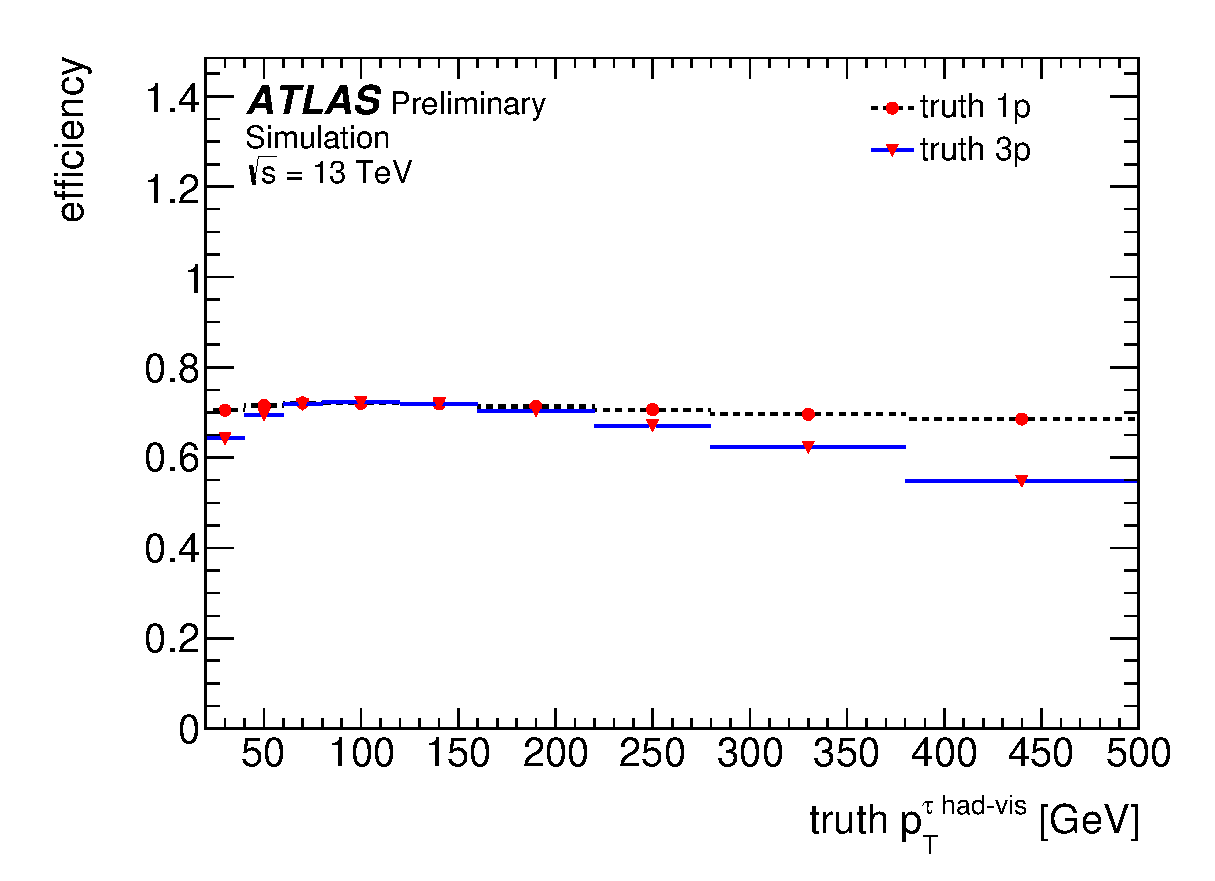
\includegraphics[width=\textwidth]{figures/tau_reco_eff.eps} 
\end{figure}
\vspace*{-\baselineskip}
\centering
Reco. Efficiency
	\end{column}
	\begin{column}{0.5\linewidth}
\begin{figure}
%  \includegraphics[width=\textwidth]{figures/tau_jet_bdt_score.pdf}
  \includegraphics[width=\textwidth]{figures/tau_ele_eff.pdf}
\end{figure}
\vspace*{-\baselineskip}
\centering
$\tau$-$e$ discrimination efficiency
	\end{column}
\end{columns}
\end{frame}

\begin{frame}{Jet to $\tau$ background}
\centering
{\large\color{blue} $q/g$ ($N^{\text{anti-}\tau}_{\text{fakes}}$)
 extrapolated to \tauvis\ ($N^\tau_{\text{fakes}}$) by Fake Factors}

\begin{outline}
\1 FF measured in two sub-regions : \tauvis-ID and anti-\tauvis-ID
\end{outline}

\vspace*{-0.5\baselineskip}

\begin{columns}[T]
	\begin{column}{0.5\linewidth}
\begin{empheq}[box=\mybox]{align}
\nonumber N^\tau_{\text{fakes}} = N^{\text{anti-}\tau}_{\text{fakes}}\times\FF
\end{empheq}
	\end{column}
	\begin{column}{0.5\linewidth}
\begin{empheq}[box=\mybox]{align}
\nonumber \FF = N_{\tau-\text{id}}/N_{\text{anti-}\tau\text{-id}} 
\end{empheq}
	\end{column}
\end{columns}

\begin{columns}
	\begin{column}{0.5\linewidth}
   \includegraphics[width=\textwidth]{figures/GetTauFFmed2D_2016.eps} 
	\end{column}
	\begin{column}{0.5\linewidth}
	\begin{outline}
\1 FF validated in region rich in QCD multi-jets
	\end{outline}
   \includegraphics[width=\textwidth]{figures/DDQCD15_QCD_MT.eps}
	\end{column}
\end{columns}

\end{frame}

\begin{frame}{Major systematic uncertainties}
\centering
{\large\bf \uline{Experimental} and \uline{theoretical}, depending on source}
%\vspace*{-\baselineskip}
\noindent\makebox[\linewidth]{\rule{\paperwidth}{0.4pt}}
%\vspace*{-\baselineskip}
\centering
{\bf\color{blue} Theoretical }
\begin{outline}
	\1  QCD renormalization and factorization scales ($\mu_R, \mu_F$), 
	\1 choice of parton distribution functions (PDF)
	\1 choice of parton shower and underlying event (PS and UE) tunes
\end{outline}

\noindent\makebox[\linewidth]{\rule{\paperwidth}{0.4pt}}
%\vspace*{-\baselineskip}
\centering
{\bf\color{red} Experimental}
\begin{outline}
\1 Dominated by uncertainties on object reco. and ID
\1 Energy scales propagated to \met
\end{outline}
\noindent\makebox[\linewidth]{\rule{\paperwidth}{0.4pt}}
\begin{columns}[T]
	\begin{column}{0.4\linewidth}
\centering
\vspace*{-\baselineskip}
\begin{table}[!h]
  \resizebox{0.9\textwidth}{!}{
\begin{tabular}{l|cc}
Variation & \ttbar\ (\%) & Signal (\%)  \\
\hline\hline
PS and UE &  16 & 10 \\
$\mu_R, \mu_F$ & 5 & 5 \\
PDF choice & 5 & 1 \\
\end{tabular}
}
\end{table}
	\end{column}
	\begin{column}{0.6\linewidth}
\centering
\vspace*{-\baselineskip}
\begin{table}[!h]
  \resizebox{0.8\textwidth}{!}{
\begin{tabular}{l|cc}
Variation & \ttbar\ (\%) & Signal (\%)  \\
\hline\hline
\tauvis\ ID efficiency & 11 & 8 \\
Jet energy scale  & 11  & 5 \\
\tauvis\ energy scale & 6 & 4 \\
\end{tabular}
}
\end{table}

	\end{column}
\end{columns}

%	\end{column}
%\end{columns}
%
\end{frame}

\begin{frame}{Results -- Event yields in the SR}
\centering
{\large\color{blue} Observed events in the SR well within predictions}
\begin{figure}
					 \includegraphics[width=0.5\textwidth]{figures/met_SR_nMinus1.eps}
   \includegraphics[width=0.5\textwidth]{figures/mT_SR_nMinus1.eps}
\end{figure}
\end{frame}

\begin{frame}{Results -- Event yields in the SR}
\begin{figure}
	 \includegraphics[width=0.33\textwidth]{figures/tauPt_SR.eps}
   \includegraphics[width=0.33\textwidth]{figures/jets_SR.eps}
   \includegraphics[width=0.33\textwidth]{figures/bJets_SR.eps}
\end{figure}
\begin{figure}
   \includegraphics[width=0.33\textwidth]{figures/tauMetPhi_SR.eps}
   \includegraphics[width=0.33\textwidth]{figures/tauEta_SR.eps}
   \includegraphics[width=0.33\textwidth]{figures/tauPhi_SR.eps}
\end{figure}
\end{frame}

\begin{frame}{Results -- Statistical interpretation, Limits}
\begin{outline}
\1 Evaluation of observed yields (and \mT\ shape) against bkg-only hypothesis performed
	\2 Could not reject bkg-only hypothesis
\1 Limits on $\sigma_{\Hplus}^{true}$ set for \mcH\ in 200$\to$2000~\GeV
\end{outline}
\vspace*{-\baselineskip}
\begin{columns}
	\begin{column}{0.5\linewidth}
\begin{figure}
					 \includegraphics[width=\textwidth]{figures/final_limits_sys_asym_limit_log.eps}
\end{figure}
	\end{column}
	\begin{column}{0.5\linewidth}
\begin{figure}
					 \includegraphics[width=\textwidth]{figures/exclusion_run2016taunu_v2_hmssm_taunu.eps}
\end{figure}
	\end{column}
\end{columns}
\centering
{\large\color{blue} In the hMSSM context, $\tan\beta=60$ values are excluded for \mcH\ in $200\to 540~\GeV$}
\end{frame}

\section{Summary}

\begin{frame}{Summary}
\begin{outline}
\1 Undertook two major projects
	\2 Search for exclusive Higgs boson
	\2 Search for charged Higgs boson
\1 Contributed to detector development
	\2 Feasibility studies on ATLAS level 1 trigger
	\2 Optimization of RoIB for level 2 ATLAS trigger
\end{outline}
\noindent\makebox[\linewidth]{\rule{\paperwidth}{0.4pt}}

\begin{outline}
\1 Found no evidence for the exclusive Higgs boson in LHC Run I data
	\2 Set the first ever limits on the production cross section
\1 Found no evidence for the charged Higgs boson in LHC Run II data
	\2 Set limits on the production cross section ($\times$ branching ratio to $\tau\nu$) 
in the 200$\to$200~\GeV\ \mcH\ range
	\2 In the hMSSM context, $\tan\beta=60$ values excluded for \mcH\ in $200\to 540~\GeV$
\end{outline}
\end{frame}

\begin{frame}{Summary}
\centering
\LARGE \emph{Thank you} 
\end{frame}

%\section{Backup Material}
\begin{frame}{Level 1 (L1) trigger -- the calorimeter}
\centering
\begin{outline}
\1 L1 trigger decision based on multiplicity of physics objects and size of \met
	\2 $e$, $\mu$, $\tau$ and jets 
\1 Calorimeters made up of cells 
	\2 however, full granularity not accessible at L1 
\1 Reconstruction of physics objects performed using groups of cells
	\2 Trigger Towers -- TT
\1 Objects distinguished based on shower shapes in the calorimeters 
	\2 e.g, a $\tau$ shower is deeper than an $e$ shower
\1 Maximum latency, 2.5 $\mu$s 
\end{outline}

Bunch crossing rate reduced from {\bf 40~MHz} to about {\bf 100~kHz}
\end{frame}

\begin{frame}{L1 upgrade -- feasibility studies (Summer 2012)}
By how much would upgrading L1 calorimeter granularity improve L1?
\vspace*{-0.5\baselineskip}
\begin{figure}
	\centering
   \includegraphics[width=0.6\textwidth]{figures/scell.pdf}
\end{figure}

\vspace*{-0.5\baselineskip}
{\color{blue}\large Using supercells can we distinguish \pizero\ and $e$ at L1?} 

%\vspace*{-0.5\baselineskip}
\begin{outline}
\1 {\bf Strategy} : Come up with variables to describe shower shapes 
	\2 e.g, ratio of energy of hottest supercell to sum of itself and two neighbors  
\end{outline}

\vspace*{-0.5\baselineskip}

\begin{empheq}[box=\mybox]{align}
R_{\eta}^{(1)} = \frac{E_{0}}{E_{+1} + E_{0} + E_{-1}}
\end{empheq}

$e$ shower narrower than \pizero\ $\longrightarrow$ expect $R_{\eta}^{(1)}$ to be  
larger for $e$ than for \pizero

\end{frame}


\begin{frame}{L1 upgrade -- feasibility studies (Summer 2012)}
\begin{outline}
\1 Generated Monte Carlo (MC) samples of either single $e$ or $\pizero$ 
\1 Simulated passage of $e/\pizero$ through ATLAS calorimeters
\1 Studied shower shapes of each using variables like $R_{\eta}^{(1)}$
	\2 More results at \href{http://www-hep.uta.edu/hep_notes/atlas/atlas_0002.pdf}{UTA hep web page}
\end{outline}
\vspace*{-0.8\baselineskip}
\begin{figure}
\centering
 \includegraphics[width=0.8\linewidth]{figures/RetaVx.png}%
\end{figure}
\vspace*{-\baselineskip}
{\color{blue}\large Cannot separate $\pizero$ and $e$ showers at L1 using supercells}
\end{frame}

\begin{frame}{L2 (HLT) upgrade --  2013$\to$2014}
Accepts/rejects events through a Regions of Interest (RoI) builder at 100 kHz
\begin{figure}
\centering
\includegraphics[width=\linewidth]{figures/trigger_l2.png}
\end{figure}
\vspace*{-\baselineskip}
 L2 and EF algorithms merged in Run II \\
 -- {\color{blue} can this setup achieve a rate of 100 kHz?}
\begin{outline}
\1 {\bf Project:} Optimize RoI Builder (RoIB) rate with Run II setup 
\end{outline}
\end{frame}

\begin{frame}{HLT -- Configuration optimization}
\centering
{\large\color{blue} Argonne National Laboratory has a test stand for HLT}
\begin{columns}
	\begin{column}{0.45\linewidth}
%\begin{outline}
%\1 13 Linux PCs carry custom-built chips as prototypes of HLT components
%\1 Performance of set-up depends on memory and hardware of PCs
%\end{outline}
\includegraphics[width=\linewidth]{figures/dcmVsRate.png}\\
\includegraphics[width=\linewidth]{figures/h_reinerOne.png}\\
	\end{column}
	\begin{column}{0.45\linewidth}
\begin{figure}
\includegraphics[width=\linewidth]{figures/ANL_RoIB-Teststand.jpg}
\end{figure}
	\end{column}
\end{columns}
Achieved a rate of {\bf$\sim$ 80~kHz} -- dependent on PC hardware 
\end{frame}




\begin{frame}{Kinematic Dists. after pre-selection}
   \includegraphics[width=0.5\textwidth]{figures/emme-CutMll-Mll-log.pdf}
   \includegraphics[width=0.5\textwidth]{figures/emme-CutMll-DPhill-log.pdf}\\
   \includegraphics[width=0.5\textwidth]{figures/emme-CutMll-MT-log.pdf}
   \includegraphics[width=0.5\textwidth]{figures/emme-CutMll-Ptll-log.pdf}
\end{frame}

\begin{frame}{Inc. $WW$ normalization}
\centering
{\large\color{blue} MC known to underestimate $q\bar{q}\rightarrow W^{+}W^{-}$ prediction}
\begin{outline}
\1 Control region similar to signal region except:
	\2 $55 < \memu < 110~\GeV$ and $\dFem<2.6$
\end{outline}
   \includegraphics[width=0.5\textwidth]{figures/emme-CutNjets-MT-lin.eps}
   \includegraphics[width=0.5\textwidth]{figures/emme-CutNjets-DPhill-lin.eps}
\begin{outline}
\1 $(20 \pm 5)\%$ more data was observed than is predicted
	\2 $1.20 \pm 0.05$(stat.) applied across the board as a scale factor
\end{outline}
\end{frame}

\begin{frame}{Inc. $WW$ + Other}
\centering
{\large\color{blue} How much inclusive $WW$ after exclusivity?}
\begin{outline}
\1 Dedicated control region with incl. $WW$ -- loosen exclusivity to allow only 1 to 4 extra tracks
	\2 Other bkg such as \Wjets, Drell-Yan, and Top irreducible
	\2 Exclusive processes well calibrated, so easy to subtract
\1 Extrapolate predictions to the 0-extra track exclusivity region 
\end{outline}
   \includegraphics[width=0.5\textwidth]{figures/emme-xtraTracks-Mll-lin.eps}
   \includegraphics[width=0.5\textwidth]{figures/emme-xtraTracks-Ptll-lin.eps}\\
\centering
Extrapolation equivalent to applying a normalization factor of 0.79 to inclusive \WW background
\end{frame}

\begin{frame}{Jet to $\tau$ background -- measured \FF, validation}
\begin{center}
   \includegraphics[width=0.45\textwidth]{figures/GetTauFFmed2D_2015.eps}
   \includegraphics[width=0.45\textwidth]{figures/GetTauFFmed2D_2016.eps} \\
   \includegraphics[width=0.45\textwidth]{figures/DDQCD15_QCD_MT.eps}
   \includegraphics[width=0.45\textwidth]{figures/DDQCD15_FFWCR_WlepMT.eps}
\end{center}
\end{frame}


\begin{frame}{Jet to $\tau$ background -- Fake Factors definition}
\centering
From CR dominated by events with $q/g$-initiated jets ($N^{\text{anti-}\tau}_{\text{fakes}}$),
 extrapolate to SR events in which the jets 
pass \tauvis\ ID ($N^\tau_{\text{fakes}}$)

\begin{columns}
	\begin{column}{0.45\linewidth}
\begin{outline}
\1 Extrapolation factors known as {\it fake factors} (\FF), where 
\end{outline}
\begin{tcolorbox}[width=\linewidth, colback=white,colframe=red,nobeforeafter,tcbox raise base,top=0pt,left=0pt,right=0pt,bottom=0pt]
\centering
$N^\tau_{\text{fakes}} = N^{\text{anti-}\tau}_{\text{fakes}}\times\FF$
\end{tcolorbox}
\begin{outline}
\1 \FF\ measured in data (next slide)
\1 Pre-test \FF\ by measuring them in \ttbar MC and assessing 
performance on \ttbar\ MC events that pass pre-selection 
\end{outline}
	\end{column}
	\begin{column}{0.55\linewidth}
   \includegraphics[width=\textwidth]{figures/Fake_MMClosure_MT.eps}
	\end{column}
\end{columns}

\end{frame}

\begin{frame}{Jet to $\tau$ background -- Fake Factors measurement}
\centering
Region in which \FF\ are {\bf measured} must be different from the CR in which they are {\bf applied}
\begin{outline}
\1 Measurement region comprises of $\tau$-id and anti-$\tau$-id sub-regions
	\2 In former jets pass $\tau$ ID and in latter they are not required to 
\end{outline}

\begin{tcolorbox}[width=\linewidth, colback=white,colframe=red,nobeforeafter,tcbox raise base,top=0pt,left=0pt,right=0pt,bottom=0pt]
\centering
$\FF = \frac{N_{\tau-\text{id}}}{N_{\text{anti-}\tau\text{-id}}}$ 
\end{tcolorbox}

\begin{outline}
\1 Here, \FF\ measured in two regions:
	\2 {\bf Multi-jet}: Dominated by events with QCD multi-jets
	\2 $\boldsymbol{\Wjets}$: Dominated by events with jets from \Wjets 
\1 Fraction of $q$-initiated jets in multi-jets roughly the same as $g$-initiated jets
\1 Jets in \Wjets\ dominated by jets from light-flavored quarks
\1 Take measurements from multi-jets as nominal and use \Wjets\ measurements to evaluate 
impact of jet substructure
\end{outline}

\end{frame}
\begin{frame}{$e/\mu$ to $\tau$ background}

\centering
{\large\color{blue} Scale factors (SF) applied to simulated events with $e/\mu$-matched \tauvis} 

\begin{outline}
\1 SF dependent on and $\eta$ and measured in $Z\to ee$ events in data
\end{outline}
\begin{columns}
	\begin{column}{0.35\linewidth}
\begin{tcolorbox}[title=\Zee Selection, width=\linewidth, colback=white,colframe=cyan,nobeforeafter,tcbox raise base,top=0pt,left=0pt,right=0pt,bottom=0pt]
\begin{enumerate}
\item One $e$, one $\tauvis$
\item 0 b-jets, $\mT<40$ 
\end{enumerate}
\end{tcolorbox}
\vspace*{-\baselineskip}
\begin{outline}
\1 $e$ tag, \tauvis\ probe
\end{outline}
\begin{empheq}[box=\mybox]{align}
\nonumber \text{SF} = \frac{\text{All sel.}}{\text{All sel.} - \tauvis \text{ sel.}}
\end{empheq}
	\end{column}
	\begin{column}{0.65\linewidth}
   \includegraphics[width=\textwidth]{figures/c7_evto_SF.eps}
	\end{column}
\end{columns}
\begin{outline}
\1 Non-\Zee\ events subtracted from data before calculation of SF
\1 Measured SF range from 0.5\% to 2.5\%, depending on $\eta$ 
\end{outline}

\end{frame}


\begin{frame}{Major systematic uncertainties}
\centering
Classified into {\it \uline{experimental}} and {\it \uline{theoretical}}, depending on source
\vspace*{1.5\baselineskip}
\begin{columns}
	\begin{column}{0.5\linewidth}
\centering
{\bf Theoretical }
\begin{outline}
\1 Dominated by uncertainties on:
\vspace*{-\baselineskip}
	\2  QCD renormalization and factorization 
scales ($\mu_R, \mu_F$), 
	\2 choice of parton distribution functions (PDF)
	\2 choice of parton shower and underlying event (PS and UE) tunes
\end{outline}
\vspace*{-0.5\baselineskip}

\begin{table}[!h]
\begin{center}
  \resizebox{0.8\textwidth}{!}{
\begin{tabular}{|l|cc|cc|cc|cc|}
\hline
\multirow{2}{*}{Variation} & \ttbar & Signal   \\
													 &        & 400~\GeV \\
\hline\hline
PS and UE &  16 & 10 \\
$\mu_R, \mu_F$ & 5 & 5 \\
PDF choice & 5 & 1 \\
\hline
\end{tabular}
}
\end{center}
\end{table}
%\begin{outline}
%\1 Impact of all these on \Wjets\ (next dominant bkg)
%less than 3\%
%\end{outline}
	\end{column}
	\begin{column}{0.5\linewidth}
\centering
{\bf Experimental}
\begin{outline}
\1 Dominated by uncertainties on object reco. and ID
	\2 Propagated to \met; propagated to trigger efficiency
\end{outline}

\vspace*{-\baselineskip}
\begin{table}[!h]
\begin{center}
  \resizebox{\textwidth}{!}{
\begin{tabular}{|l|cc|cc|cc|cc|}
\hline
\multirow{2}{*}{Variation} & \ttbar & Signal   \\
													 &        & 400~\GeV \\
\hline\hline
\tauvis\ ID efficiency & 11 & 8 \\
\tauvis\ energy scale & 6 & 4 \\
\tauvis\ reconstruction efficiency &  3 & 2 \\
\tauvis-lepton OLR & 1 & 2 \\
\hline 
Jet energy scale  & 11  & 5 \\
$b-$tagging efficiency  & 2 & 2  \\
\met\ soft term scale/resolution & 2 & 2 \\
Trigger efficiency & 3 & 1 \\ 
\hline
\end{tabular}
}
\end{center}
\end{table}
	\end{column}
\end{columns}

\end{frame}

\begin{frame}{Uncertainties impact on limits}
\centering
{\bf Impact of various sources of uncertainty on
      the expected 95\% CL exclusion limit}
\begin{table}[h!]
 \begin{center}
  \resizebox{\textwidth}{!}{
   \begin{tabular}{|l|l|cc|}
\hline
Category    &  Source of systematic & \multicolumn{2}{c|}{Impact on the expected limit (in \%)} \\
    &  uncertainty & $m_{H^+} = 200~\GeV$ & $m_{H^+} = 1000~\GeV$ \\
     \hline\hline
	\multirow{5}{*}{Experimental} & luminosity  &  $\phantom{0}1.5$   &  $\phantom{0}0.9$ \\
     & trigger  &  $<0.1$  &  $<0.1$ \\
     & $\tau_{\text{had-vis}}$  &  $\phantom{0}1.0$   &  $\phantom{0}1.4$ \\
     & jet  &  $\phantom{0}3.0$   &  $\phantom{0}0.2$ \\
     & $\met$  &  $<0.1$   &  $<0.1$ \\
     \hline
 \multirow{1}{*}{Fake factors} &  \FF  &  $\phantom{0}0.8$   &  $\phantom{0}4.7$ \\
     \hline
 \multirow{2}{*}{Signal and background models}    & $t\bar{t}$ modelling   &  $\phantom{0}13.2$   &  $\phantom{0}3.5$ \\
     & $H^+$ signal modelling  &  $\phantom{0}1.4$   &  $\phantom{0}1.4$ \\
     \hline
   \end{tabular}
}
  \end{center}
\end{table}
\centering
Largest impact was from modelling \ttbar\ background processes
\end{frame}



\end{document}
